
\section{HIJSON Toolkit}\label{hijson-toolkit}

The HIJSON Toolkit is a software module that implements common
operations and transformations on HIJSON documents. Written in
\emph{JavaScript} language, this software module has been built to be deployed in the web
environment. It is \emph{modular} and entirely \emph{isomorphic},
i.e.~can run on the server as well as on every client. Working in the
web environment, the Toolkit benefits of the ``fertility'' commonly concerning the
software development in this field: for example, it takes advantage of libraries and
frameworks such as \emph{React}, ``the JavaScript library for building
user interfaces'' by Facebook, and as \emph{Three.js}, the current de-facto standard to deal
with \emph{WebGL} tecnologies.

The Toolkit executes the instantiation and extension logic of a HIJSON
document, and provides a multistage transformation pipeline that, according to the requirements,
can be used either entirely or only in part.

\subsection{Processing pipeline}\label{hijson-processing-pipeline}

The HIJSON processing pipeline implements the sequence of preliminary
transformations that have to be applied to a HIJSON document before any
further operation. It is not strictly required to complete each stage of
the pipeline: the exit stage depends on the specific use case.

The application of the transformation pipeline has a double aim. The first one
consists in generating the graph of valid paths among all the interesting
HIJSON elements. The second objective is the generation of one \emph{GeoJSON}
document for each storey of the building described by the HIJSON document. In
this way a bidimensional layout  can be provided for every level of the building, 
and visualized through any compliant GeoJSON viewer.

The HIJSON processing pipeline is composed by 6 elaboration stages, denoted as \emph{validation}, \emph{georeferencing}, \emph{parsing}, \emph{graph
paths generation}, \emph{2D layers generation}, \emph{marshalling}. The pipeline of transformations and the output of each stage are shown in Figure~\ref{fig:pipeline}.

\begin{figure}[!htbp]
\centering
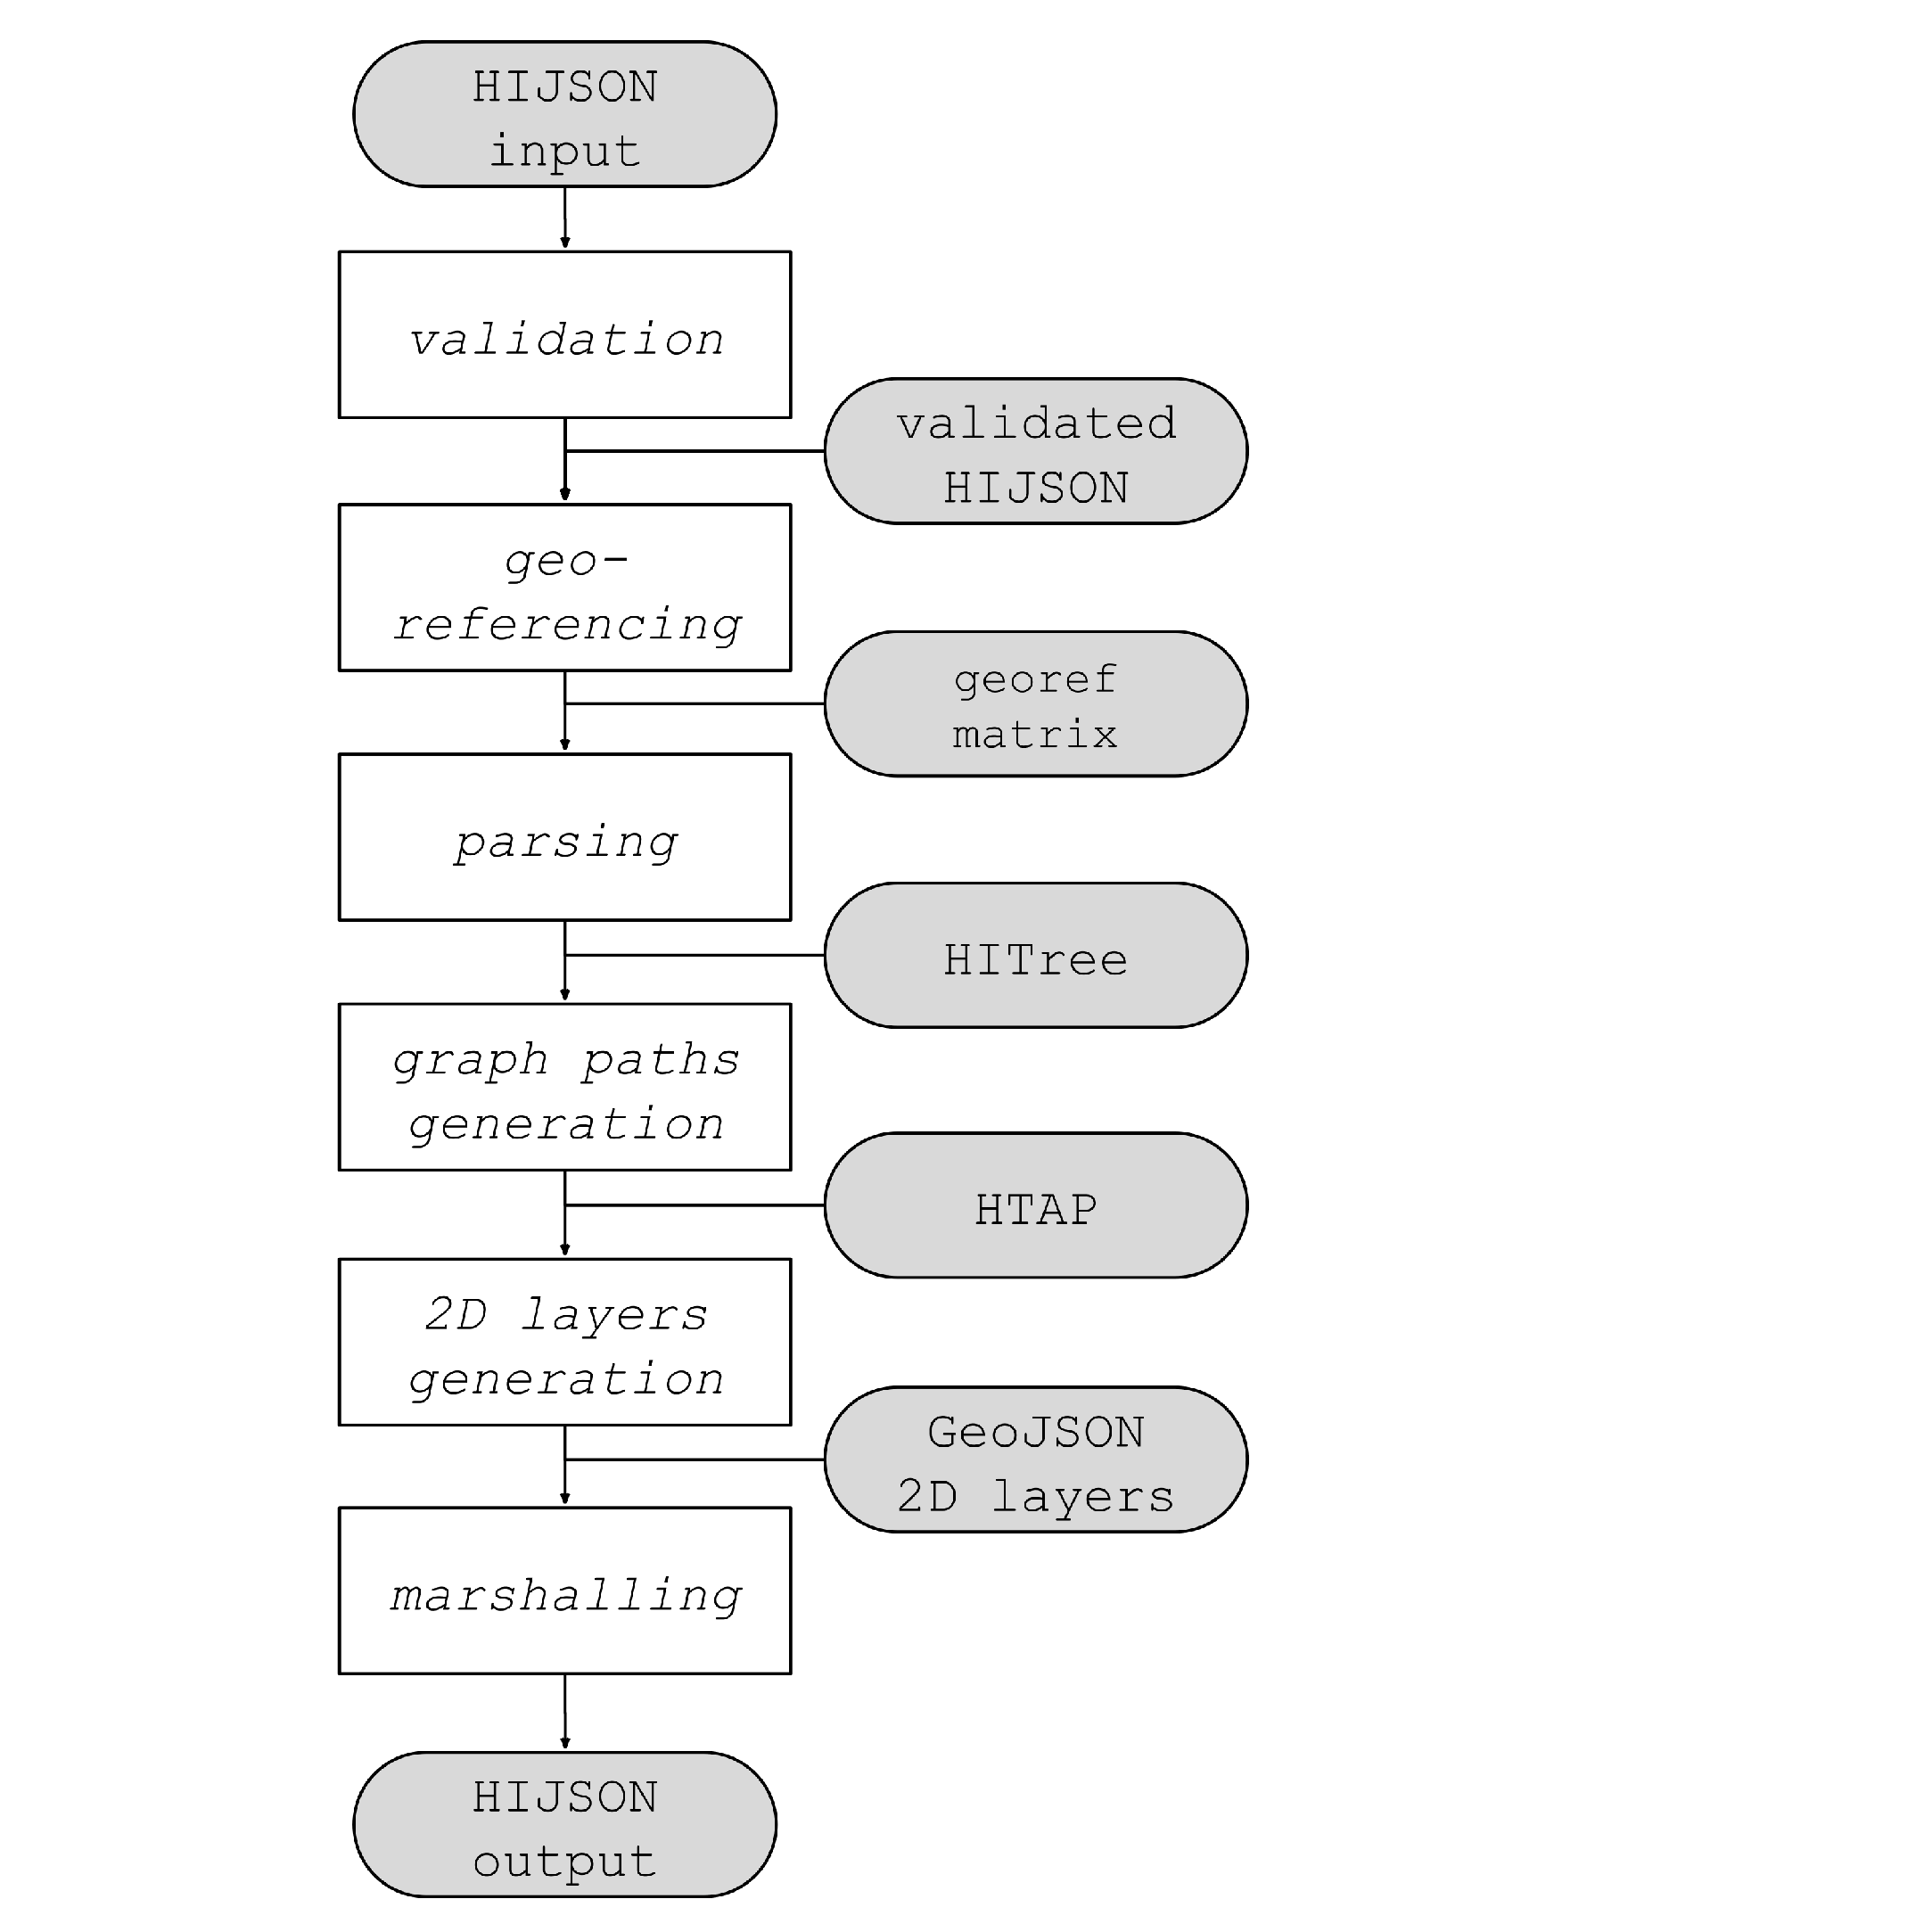
\epsfig{file=images/pipeline.eps, height=0.4\textwidth}
\caption{HIJSON processing pipeline}
\label{fig:pipeline}
\end{figure}

\begin{enumerate}
\def\labelenumi{\arabic{enumi}.}
\itemsep1pt\parskip0pt\parsep0pt
\item
 \textit{\texttt{validation}} - The first one is the validation stage. In
  order to begin with the effective transformations the input HIJSON  document
  must be compliant with both the syntax format and the structural requirements.   In the
  case the validation stage fails, processing aborts and does not continue to
  following stages. If this stage successes, then the output for the next stage is a
  validated  HIJSON.

\item
 \textit{\texttt{georeferencing}} - In the second stage, in order to allow
 for continuous outdoor/indoor navigation, the system needs to compute
 the georeference matrix, a linear operator able to transform local
 coordinates into global coordinates (world coordinate
 system---latitude and longitude angles) and viceversa. This task is
 accomplished by solving a linear system obtained from information
 contained in HIJSON configuration part and precisely from the
 correnspondance of three real word points to three points included
 into the HIJSON document.
\item
 \textit{\texttt{parsing}} - The parsing stage takes the validated and
 georeferenced HIJSON as its input, that as illustrated before can be
 thought of as a list of HIJSON Elments, parses them and produces an
 istance of the HIJSON Tree. The HIJSON Tree is an object in memory
 representing the hierarchical structure of the building described
 by the HIJSON document.
\item
 \textit{\texttt{graph of paths generation}} - The fourth stage is in char\-ge
 of the generation of the graph of paths. The algorithm to achieve such a 
 goal is introduced in Section~\ref{sec:paths}. The graph of paths can be used to compute valid directions between pairs of points of
 interest inside the building model. Once the graph of paths has been computed, the
 input HIJSON Tree is augmented with paths information, becoming what
 has been called an HTAP (HIJSON Tree Augmented with Paths).
 Augmentation always takes place when leaf nodes added as children of a
 specific level (e.g. ``room'').
\item
 \textit{\texttt{2D layers generation}} - The fifth stage concerns the
 generation of GeoJSON \emph{layers}. For each storey of the building, the Toolkit generates a
 GeoJSON layer that can be used for the creation of a 2D map. Each layer
 contains only the children of a `level' node of the HIJSON Tree. 
 The presence of a specific element inside the layer can be finely tuned 
 by means of a Boolean value. Every element has geographical coordinates, 
 calculated by multiplication times the current transformation matrix associated during the tree traversal to the local
 coordinates of the HIJSON Element.
\item
 \textit{\texttt{marshalling}} - The last stage is responsible of executing
 a serialization of the the transformed data. Tasks like breaking
 dependency-loops and stringification are performed. This stage is
 mainly useful  server-side, as the output is there stored ready to be
 served to any requiring client.
\end{enumerate}

\subsubsection{Automatic generation of valid paths}\label{algorithmics-automatic-generation-of-valid-paths}\label{sec:paths}

The fourth stage of the processing pipeline is responsible for the
generation of a graph of valid paths through the entire model
represented by the intput HIJSON document. The graph generated according
to the algorithm described in the following, although non optimal,
ensures a complete coverage of the surface while limiting the number of
generated nodes. The resulting graph is weigthed on the edges with nodes
distances. Each graph node may represent either:

\begin{enumerate}
\def\labelenumi{\alph{enumi}.}
\itemsep1pt\parskip0pt\parsep0pt
\item
 a \emph{standard path node}, i.e.~a junction node or possibly an endpoint of a
 path;
\item
 a \emph{connection node}, used as subproblem composing element in the divide et
 impera approch adopted (as described below).
\item
an \emph{element node} i.e.~HIJSON Element (whose HIJSON Class explicitly grants
 his presence in the graph), typically an endpoint of a path;
\end{enumerate}

The graph of paths allows for calculations of directions between any two given
nodes. Although different approaches have been explored \cite{6999103}, 
a very classical solution has been selected in this case, so directions 
are actually computed client-side by applying the Dijkstra algorithm to the graph. 

Taking advantage of the hierarchical structure of the HIJSON document,
and according to the divide et impera approach, the problem of 
paths generation is splitted in several sub-problems, which consist in
the computation of the sub-graphs relative to each individual space, more generally a single room. The sub-graphs are then linked together through the
connection nodes (which in most cases represent doors). The resolution
of each sub-problem (as depicted in Figure~\ref{fig:graph-generation}), 
is composed by 4 steps:

\begin{enumerate}
\def\labelenumi{\arabic{enumi}.}
\itemsep1pt\parskip0pt\parsep0pt
\item
 Computation of the walkable area of the space: this task is
 accomplished by subtracting the shape of the obstacles from the area
 of the space; the result is tipically a surface with holes;
\item
 Triangulation of the walkable area: the computed surface is
 triangulated taking into account the presence of holes;
\item
 Identification of graph nodes: for each triangle side completely
 internal to the area, its midpoint is selected as standard path node;
\item
 Junction of nodes: nodes relative to the same triangle are then linked
 pairwise; both element nodes and connection nodes (i.e.~doors) are
 linked to the nearest node of the space (i.e.~room).
\end{enumerate}

\begin{figure*}[!htbp]
 \centering
 \begin{subfigure}[b]{0.235\textwidth}
 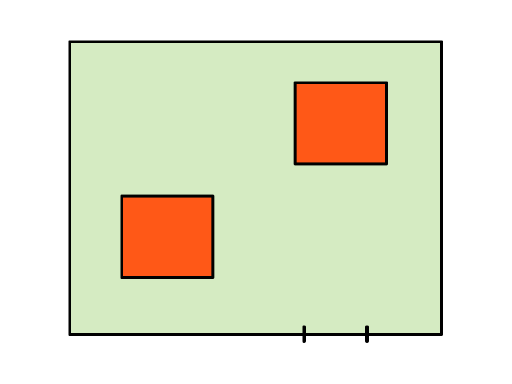
\includegraphics[width=\textwidth]{images/graph-generation/single/graph-generation-1}
 \caption{}
 \label{fig:graph-generation-a}
 \end{subfigure}
 ~
 \begin{subfigure}[b]{0.235\textwidth}
 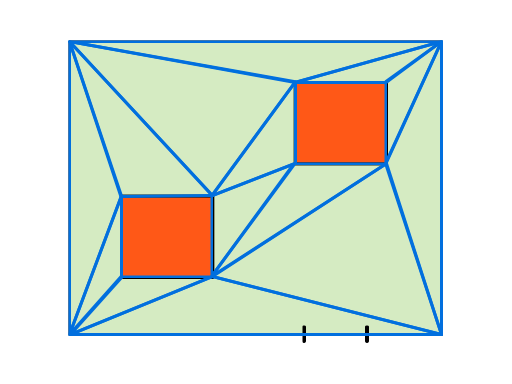
\includegraphics[width=\textwidth]{images/graph-generation/single/graph-generation-2}
 \caption{}
 \label{fig:graph-generation-b}
 \end{subfigure}
 ~
 \begin{subfigure}[b]{0.235\textwidth}
 
\includegraphics[width=\textwidth]{images/graph-generation/single/graph-generation-3}
 \caption{}
 \label{fig:graph-generation-c}
 \end{subfigure}
 ~
 \begin{subfigure}[b]{0.235\textwidth}
 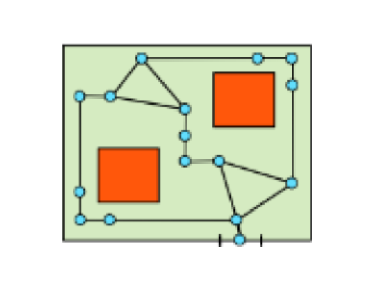
\includegraphics[width=\textwidth]{images/graph-generation/single/graph-generation-4}
 \caption{}
 \label{fig:graph-generation-d}
 \end{subfigure}
 
 \caption{graph of paths generation: 
 (a) detection of obstacles and computation of walkable area; 
 (b) triangulation of walkable area; 
 (c) identification of graph nodes area; 
 (d) junction of nodes.
 }
 \label{fig:graph-generation}
\end{figure*}

\subsection{HIJSON Class definition}\label{hijson-class-definition}

To make better use of the possibilities offered by the HIJSON Toolkit and by the
HIJSON document format, some custom dynamic behaviours can be described. These
behaviours encapsulate the specificities relative to communication
protocols with the sensors, as well as to features of user interaction. The
interface for such behaviours is the HIJSON Class.

\begin{figure}[!h]
\centering
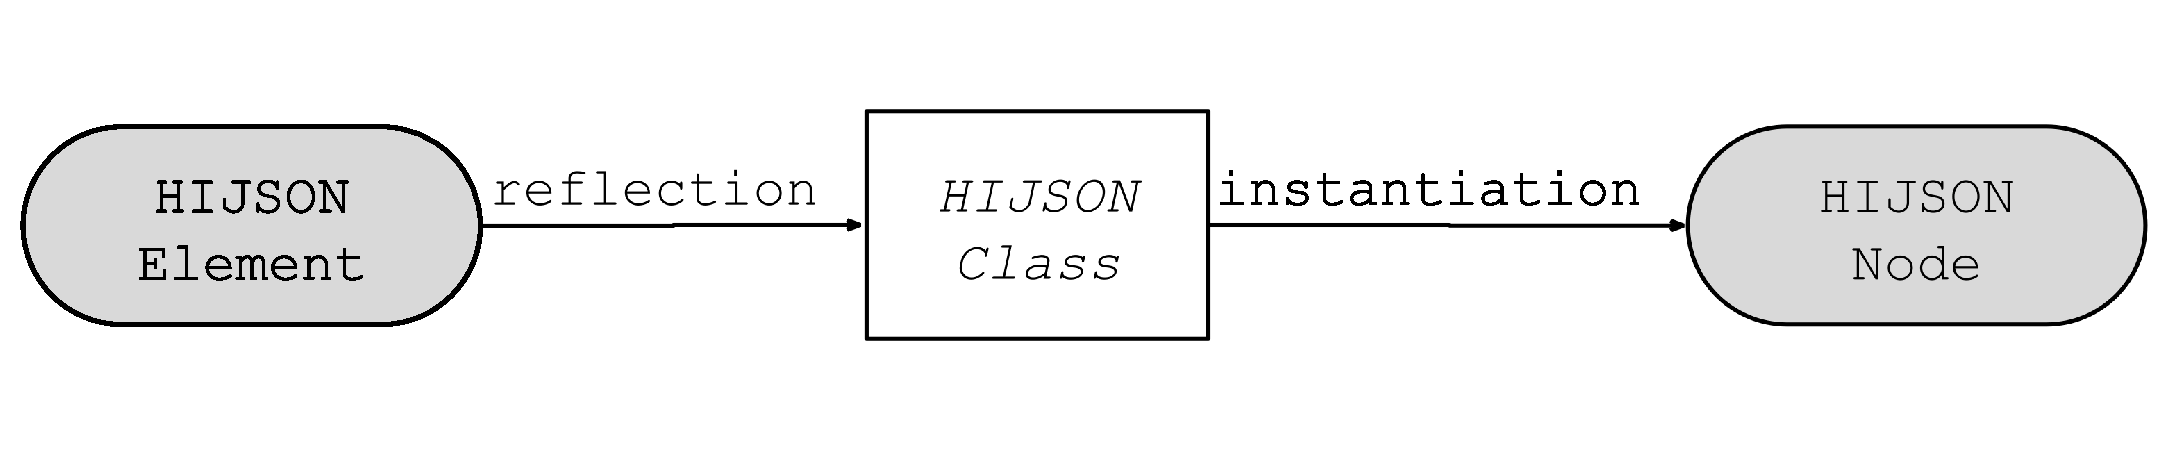
\epsfig{file=images/element-class-node.eps, width=0.44\textwidth}
\caption{HIJSON Element/Class/Node relashionship}
\label{fig:elem-class-node-rel}
\end{figure}

Evary HIJSON Element of the input HJSON document has a dynamic
counterpart, a running instance called \emph{HIJSON Node}, instantiated
according to the corresponding HIJSON Class via reflection methods (see
Figure~\ref{fig:elem-class-node-rel}).

To specify a new \emph{HIJSON Class} means to extend the Toolkit to deal with a
new class of HIJSON Element.
To extend the toolkit in order to deal with a new class of HIJSON Element is
required to specify a new HIJSON Class, by defining the following
properties and methods:

\begin{itemize}
\item
 \texttt{in\_graph}: a Boolean value to express if the element is an
 approachable point in the graph of paths;
\item
 \texttt{in\_2D\_map}: a Boolean value to express if the element must 
 be shown in the 2D map;
\item
 \texttt{get2DStyle()}: a method that returns the 2D map appearence of
 the element, essentially HTML and CSS code;
\item
 \texttt{get3DModel()}: a method that returns the 3D model appearence of
 the element, i.e.~an instance of \texttt{Obj\-ect\-3D} of the \emph{THREE.js} 
 framework;
\item
 \texttt{getWidget()}: a method that returns the information widget, a
 \emph{React} component;
\item
 \texttt{getProxy()}: a method that returns the server-side proxy which
 encapsulate the IoT sensor communication protocol, i.e.~a \emph{Node.js}
 module.
\end{itemize}

User's needs for new indoor elements, greatly different sensor equipments,
alternative representations of 2D or 3D viewports are accepted by the
definition of new HIJSON Classes, that so provide single-point
custom extensions of the Toolkit capabilities.


\begin{figure*}[htb]
\centering
% 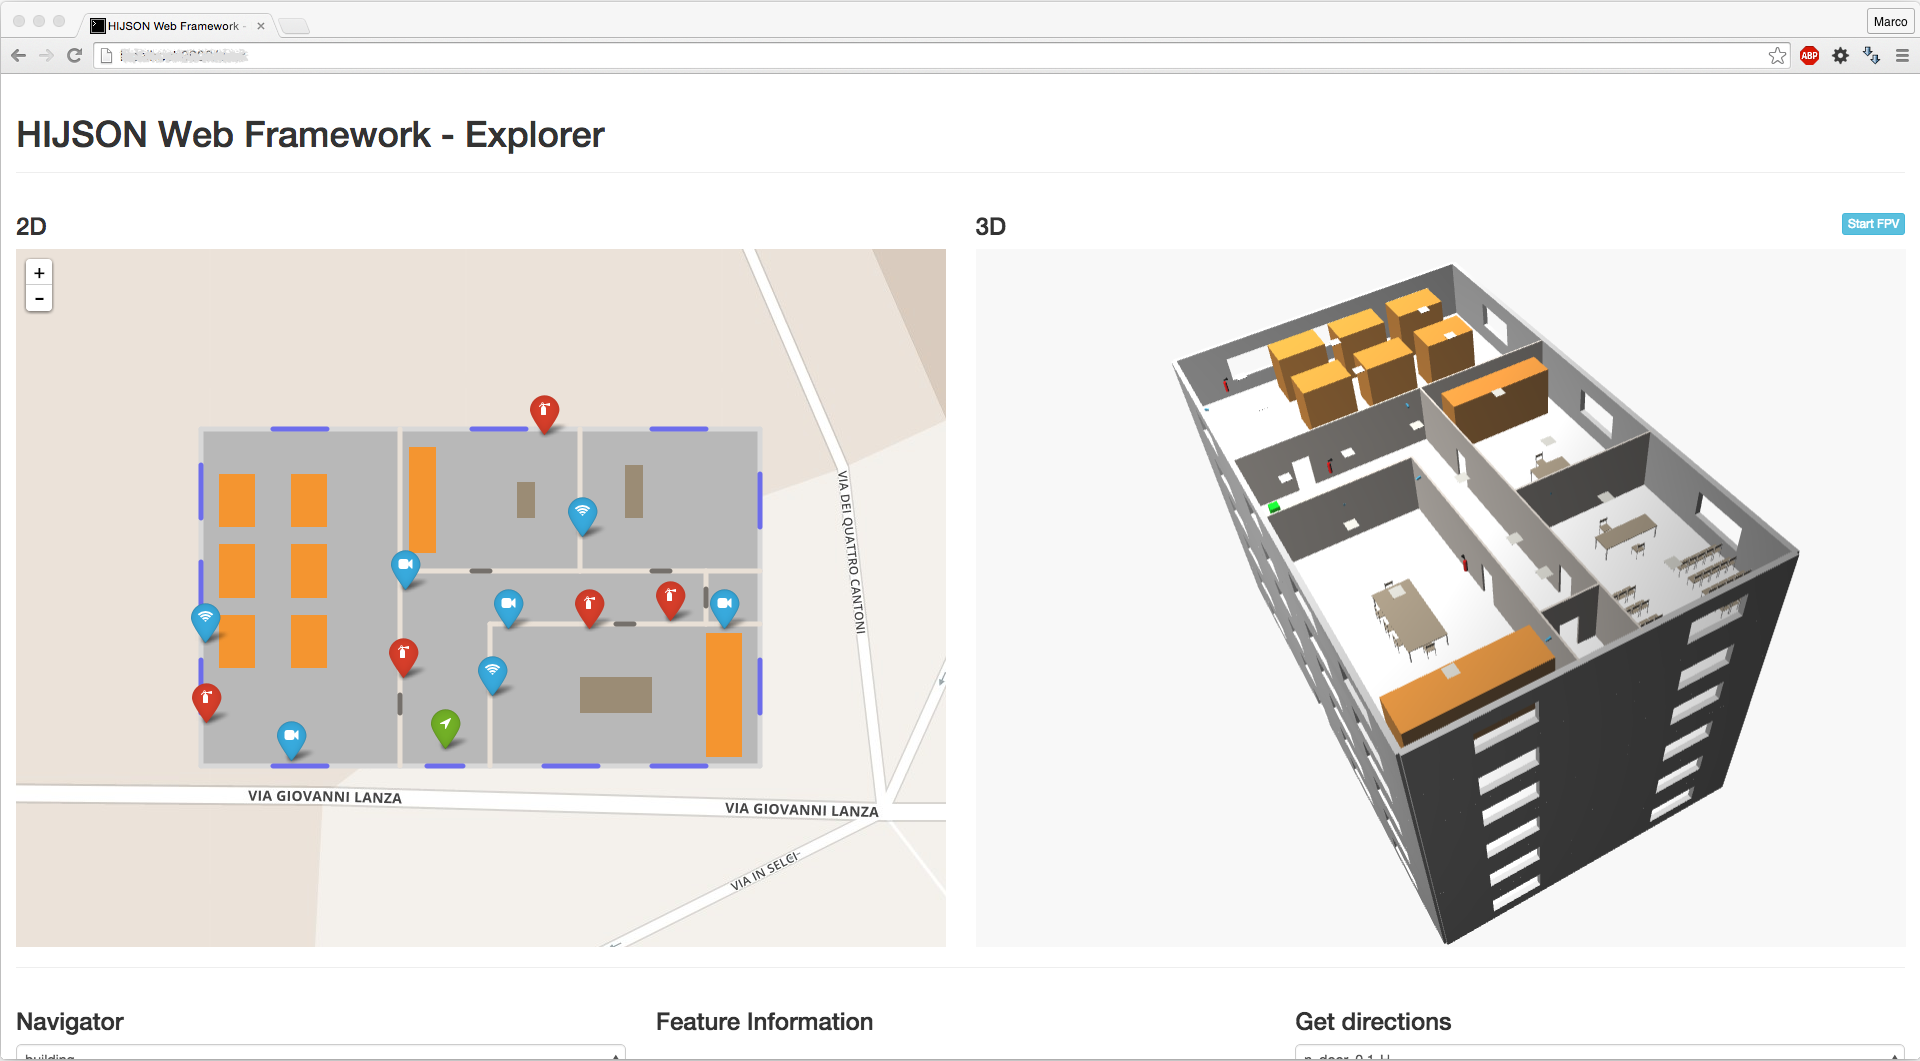
\includegraphics[width=\textwidth]{images/web_framework_1.png}
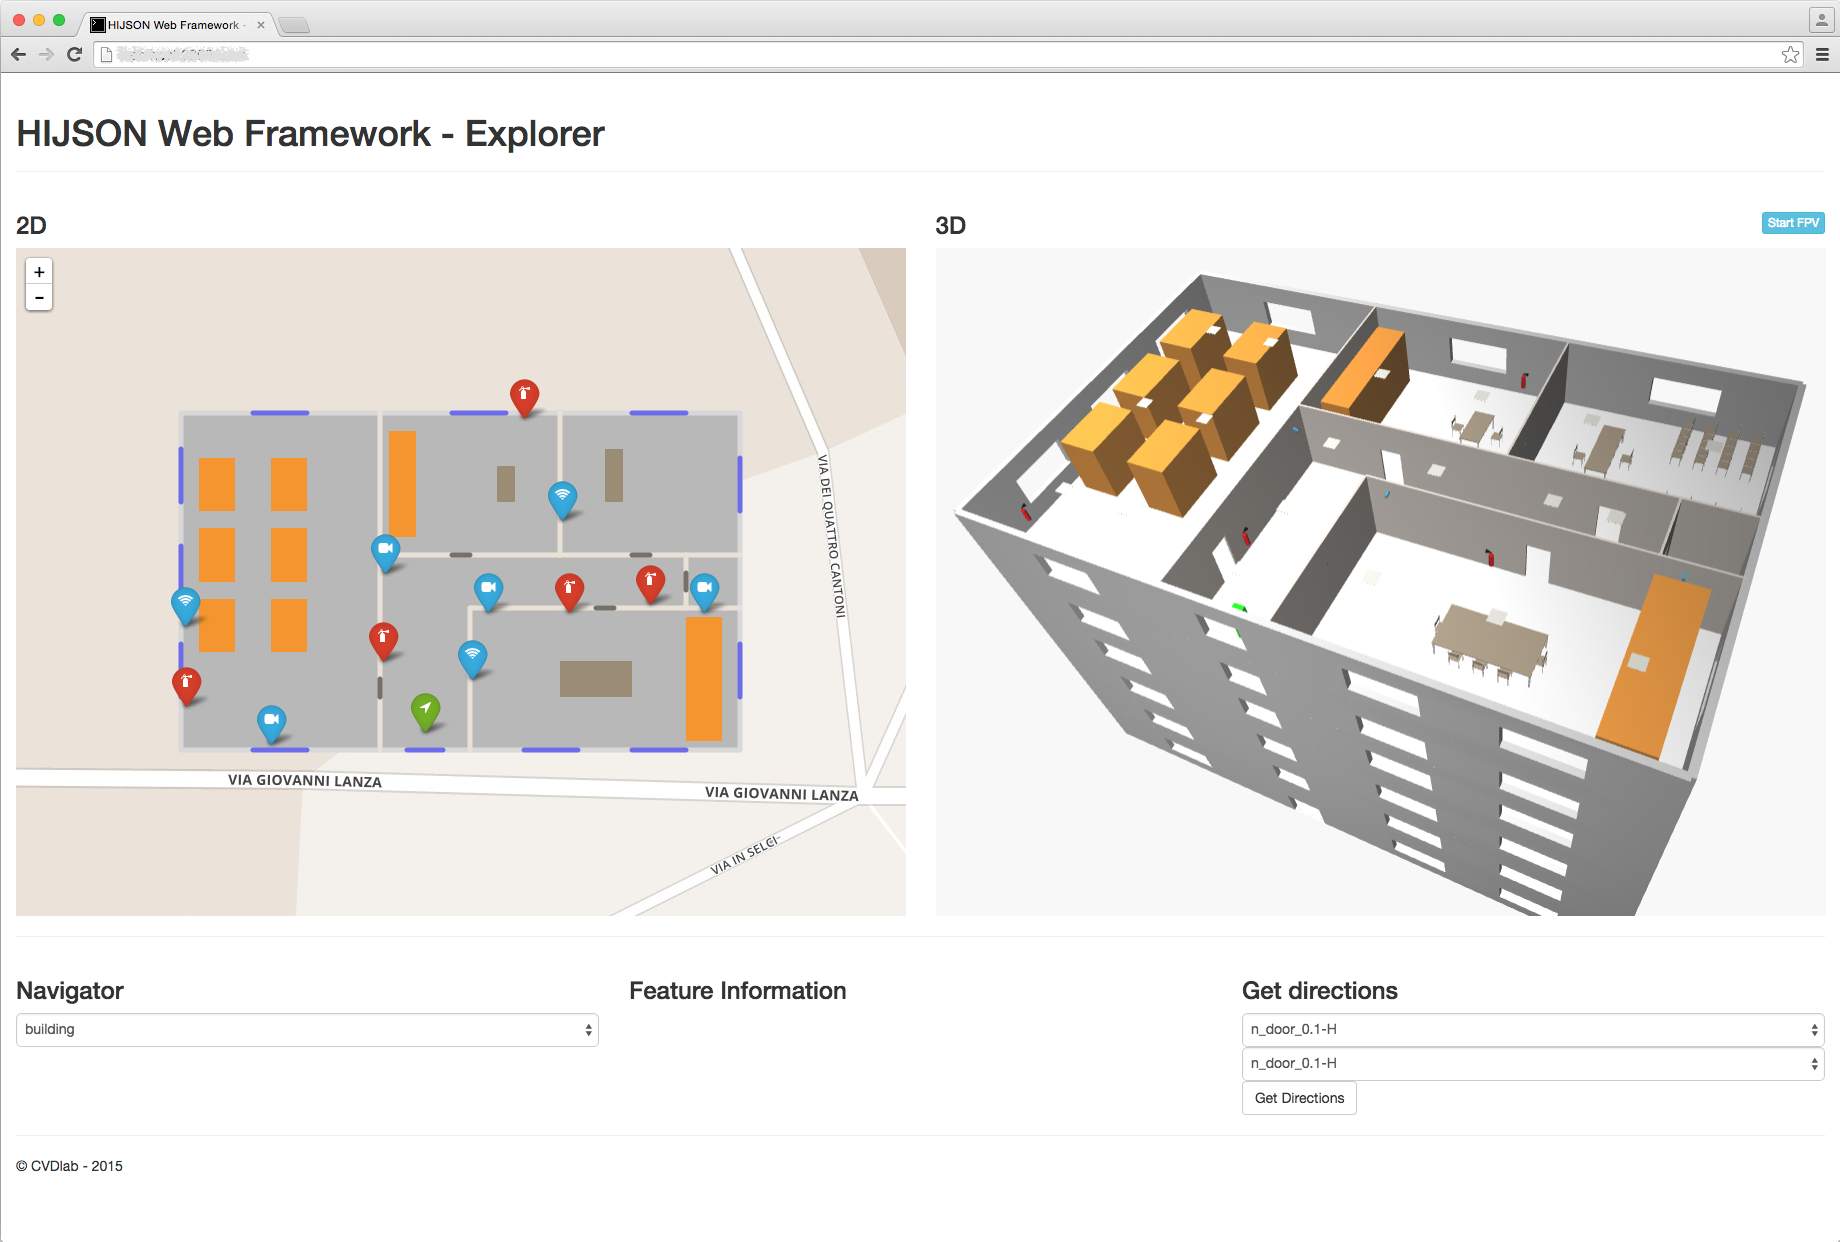
\includegraphics[width=\textwidth]{images/web_framework_2.png}
\caption{HIJSON Web Framework UI}
\label{fig:web-framework-ui}
\end{figure*}
